\documentclass[twocolumn,10pt]{jsarticle}
\usepackage[dvipdfmx]{graphicx}
\usepackage[top=19truemm,bottom=18truemm,left=14.5truemm,right=14.5truemm]{geometry}
\usepackage{listings}
\lstset{
basicstyle={\small},% 
identifierstyle={\small},% 
commentstyle={\small\ttfamily \color[rgb]{0,0,0}},% 
keywordstyle={\small\bfseries \color[rgb]{0,0,1}},% 
ndkeywordstyle={\small},% 
stringstyle={\small\ttfamily}, 
frame={tb}, 
breaklines=true, 
columns=[l]{fullflexible},% 
numbers=left,% 
xrightmargin=0zw,% 
xleftmargin=3zw,% 
numberstyle={\scriptsize},% 
stepnumber=1, 
numbersep=1zw,% 
morecomment=[l]{//}% 
}
\makeatletter
 \def\@maketitle{%
   \newpage\null
   \begin{center}%
     \let\footnote\thanks
     {\LARGE \@title \par}%
     \vskip 1.0em
     {\large
       \lineskip .5em
       \begin{tabular}[t]{c}%
         \@author
       \end{tabular}\par}%
     \vskip 1em
     {\large \@date}%
   \end{center}%
   \par\vskip 0.5em
   \ifvoid\@abstractbox\else\centerline{\box\@abstractbox}\vskip1.5em\fi
 }
\makeatother
\makeatletter
 % sectionの下マージンを小さく
 \renewcommand{\section}{%
   \@startsection{section}{1}{\z@}%
   {0.4\Cvs}{0.1\Cvs}%
   {\normalfont\large\headfont\raggedright}}
\makeatother
\setlength\intextsep{10pt}
%
% ここでタイトルの設定をします
%
% 自分の名前
\author{佐原 優衣	 榊原 一紀	 中村 正樹	 	 富山県立大学}
\date{}
% タイトル
\title{UPPAALを用いた自動運転車の\\群制御アルゴリズムのモデル化と検証}
%
%----- begin document
%
\begin{document}
\maketitle
\thispagestyle{empty}
\section{研究背景と目的}
%1--
近年,自動運転技術は発達し続けている。道路交通が自動運転車のみで構成される都市空間を考える。多数の自動運転車が発生する都市空間では,道路上の車両密度が高くなるため,様々な問題が発生する可能性がある。したがって自動運転車群に対する効率的な群制御アルゴリズムが必要となる。本研究では,自動運転車で構成された都市空間における群制御アルゴリズムをモデル化し,その性質をモデル検査技術によって形式的に検証する手法を提案する。

モデル検査は,システム上で起こり得る状態を網羅的に調べることにより設計の誤りを発見する自動検証手法の一種である。モデル検査手法は,図\ref{ModelV}に示すように,システムの振る舞いの設計,および検証したい性質をそれぞれモデル化し,ツールを用いて,システムが性質を満たしているかを調べる。本研究では,時間オートマトンによる時間制約検証が行えるモデル検査ツールUPPAAL\cite{no1}を採用する。
	\begin{figure}[htbp]
	\centering
	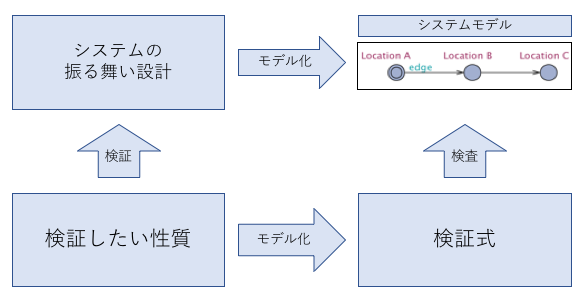
\includegraphics[width=65mm]{ModelVerification.png}
	\caption{モデル検査とは}
	\label{ModelV}
	\end{figure}

UPPAALはGUIベースのモデリング環境を提供している。このため,作成したシステムモデルが直感的に把握しやすい。入力したシステムモデルに対して,GUIベースでシミュレーション実行とモデル検査による自動検証が可能である。シミュレーション画面では,各プロセスの現在状態と変数の値,状態遷移図とメッセージシーケンスが表示される。
%2--
\section{UPPAALを用いたモデル化と検証}
UPPAALを用いて交差点を通過する1台の車両の時間オートマトンを作成する(図\ref{Simple})。車両は交差点進入前,交差点通過中,通過後の3つの状態に分けられる。交差点進入時に使用権を獲得し,通過中状態から通過後状態に遷移時に使用権を解放する。状態遷移可能条件を時間とすることによって,通過にかかる時間や何秒前に使用権を獲得しなければならないかを検証できる。
\begin{figure}[htbp]
\centering
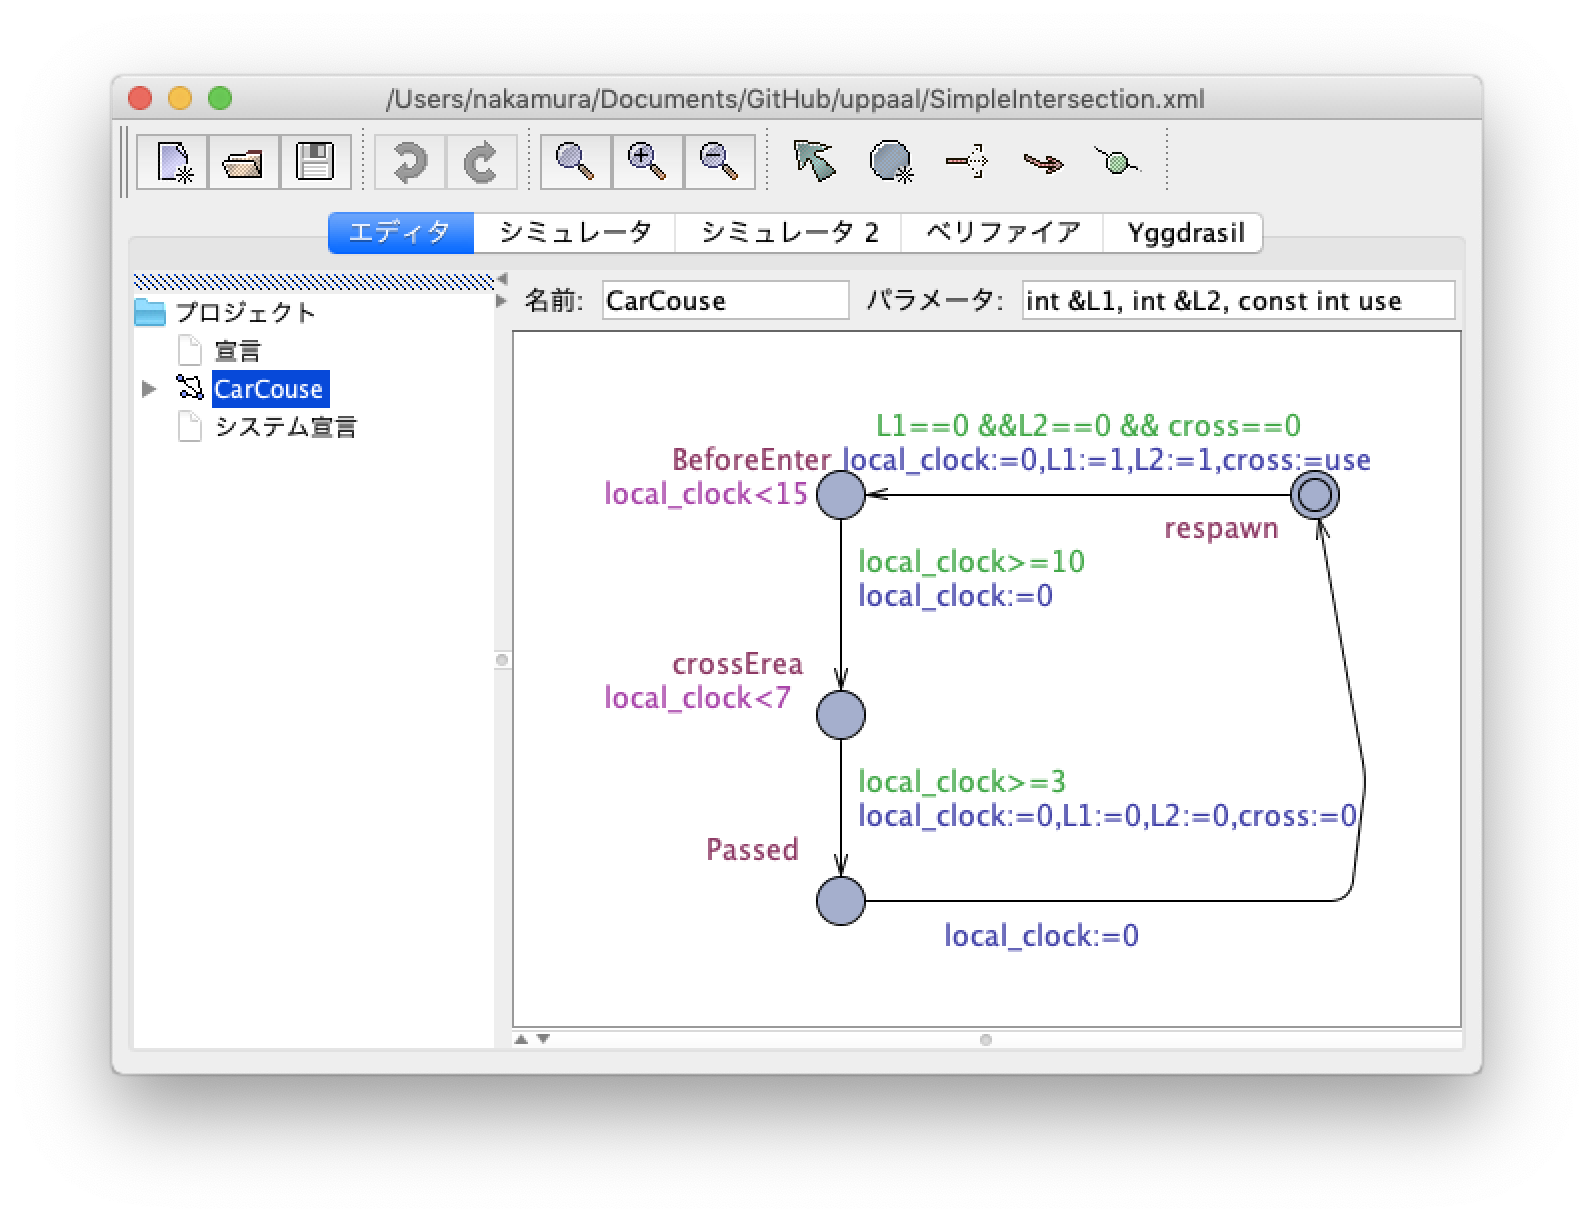
\includegraphics[width=65mm]{Simple.png}
\caption{車両一台の交差点通過モデル}
\label{Simple}
\end{figure}

1台の車両の挙動は直進も右折も左折も同様なため,同一の挙動定義のテンプレートから複数の車両のオートマトンを作成する。東西南北それぞれ直進,左折,右折の全部で12のオートマトンを合成する。

この12台の車両は任意のタイミングで交差点の進入を試み,使用権を獲得できる車両が進入前状態に遷移する。交差点の使用権は,進行方向が平行な車両は同時通過可能とし,進行方向が垂直となる車両は先に鍵を取得した方が進入する。また右折同士は衝突の可能性があるため,右折同士も同様には先に使用権を取得した方通過する。

どれだけ時間が経過しても,いずれの車両も遷移できないデッドロックが起きないかどうかを検証した。検証にかかる時間は11秒前後であった。
\section{まとめ}
本研究では,UPPAALを用いた自動運転車群制御アルゴリズムのモデル化と検証の手法を提案した。単一の交差点においては車両の挙動をモデル化し,デッドロックや通過時間を検証することができた。複数の交差点から構成される都市空間のモデルを作成し検証することが今後の課題である。
\begin{thebibliography}{1}
\bibitem{no1}{\small 長谷川哲夫,田原康之,磯部祥尚, UPPAALによる性能モデル検証ーリアルタイムシステムのモデル化と検証ー, 近代科学社, 2012.}
\end{thebibliography}
%
\end{document}
